% \documentclass[11pt,twoside,a4paper]{article}
% \usepackage{times}

% \usepackage{xeCJK}

% \setmainfont{Times New Roman}

% \setCJKmainfont{Songti SC}
\documentclass[10pt]{ctexart}
% \usepackage[UTF-8]{ctex}
\usepackage{amsmath}
\usepackage{amsthm} % 根据 amsthm 的手册, amsthm 的加载要在 amsmath 之后
\usepackage{amssymb}  %为了能使用\mathbb{H} 
\usepackage{booktabs}
\usepackage{multirow}
\usepackage{tabularx}
\usepackage{xcolor}
\usepackage[colorlinks,linkcolor=blue]{hyperref} % 使用超链接
\usepackage{pdfpages}
\usepackage{geometry}
\geometry{a4paper,scale=0.7}
\usepackage{graphicx} %插入图片的宏包
\usepackage{float} %设置图片浮动位置的宏包
\usepackage{subfigure} %插入多图时用子图显示的宏包
\usepackage{graphicx}

\usepackage{listings}

\lstset{
 columns=fixed,       
 numbers=left,                                        % 在左侧显示行号
 numberstyle=\tiny\color{gray},                       % 设定行号格式
 frame=none,                                          % 不显示背景边框
 backgroundcolor=\color[RGB]{245,245,244},            % 设定背景颜色
 keywordstyle=\color[RGB]{40,40,255},                 % 设定关键字颜色
 numberstyle=\footnotesize\color{darkgray},           
 commentstyle=\it\color[RGB]{0,96,96},                % 设置代码注释的格式
 stringstyle=\rmfamily\slshape\color[RGB]{128,0,0},   % 设置字符串格式
 showstringspaces=false,                              % 不显示字符串中的空格
%language=c++,                                        % 设置语言
}

\newtheorem{definition}{定义}
\newtheorem{lemma}{引理}
\newtheorem{theorem}{定理}

\usepackage{comment,enumerate,multicol,xspace}

  \newcounter{mnote}
  \setcounter{mnote}{0}
  \newcommand{\mnote}[1]{\addtocounter{mnote}{1}
    \ensuremath{{}^{\bullet\arabic{mnote}}}
    \marginpar{\footnotesize\em\color{red}\ensuremath{\bullet\arabic{mnote}}#1}}
  \let\oldmarginpar\marginpar
    \renewcommand\marginpar[1]{\-\oldmarginpar[\raggedleft\footnotesize #1]%
    {\raggedright\footnotesize #1}}

\title{高效密码运算算法课程笔记}
\author{谢文进}
\date{\today}
\begin{document}
\maketitle
\tableofcontents
\section{快速椭圆曲线翻倍和加法算法和乘法算法}
\subsection{椭圆曲线}
有限域上椭圆曲线的定义如下:
\begin{definition}[\textbf{椭圆曲线}]
    $\mathbb{Z}_p(p>3)$上的椭圆曲线指满足以下条件的对所有对$(x,y) \in \mathbb{Z}_p$的集合
    \begin{equation}
        y^2 \equiv x^3 + a \cdot x + b \mod p
    \end{equation}
    以及一个无穷大的虚数点$\mathcal{O}$,其中$a,b \in \mathbb{Z}_p$并且满足条件$4 \cdot a^3 + 27 \cdot b^2 \neq 0 \mod p$.
\end{definition}
有限域上的椭圆曲线的点和加法运算构成一个有限交换群$S$.

\subsection{快速椭圆曲线翻倍和加法算法}
\begin{itemize}
    \item 记$p$是一个素数
    \item $g$是阶数为$p$的循环群中的一个群元素,则$g \times p = 1_G$.
    \item 将$g$看作是椭圆曲线上的一个点,计算$[n]g$(意思就是$n$个g相加)
    \begin{itemize}
        \item 传统方式:$(((g + g) + g)) + g + \cdots$,这种方式会进行$n-1$次加法运算。
        \item 另一种方式:翻倍计算$2^kg$,
        $$
        \mathcal{P}_0 = g; \mathcal{P}_1 = 2 \mathcal{P}_0; \mathcal{P}_j = 2 \mathcal{P}_{j-1}; \cdots
        $$
    \end{itemize} 
\end{itemize}
首先,将$n$写成二进制形式,表示为:
\begin{displaymath}
    n = e_0 + e_1 \cdot 2 + e_2 \cdot 2^2 + \cdots + e_{\lambda - 1} \cdot 2 ^{\lambda - 1}, \quad \lambda - 1 = t.
\end{displaymath}
算法为
\begin{lstlisting}
    Q = g
    For i = 1 to t
        Q = 2Q (实际上每次 Q = 2^i * g)
        if ei = 1 R = R + Q (如果ei = 0, 这里就可以减少计算)
    Return R(ng)
\end{lstlisting}

\subsection{快速椭圆曲线乘法群算法}
对于一个乘法群$G$,$g \in G$,如果$n = \sum e_i 2^i$,则
\begin{displaymath}
    g^n = g^{\sum e_i 2^i} = \prod g^{e_i 2^i}= \prod (g^{2^i})^{e_i}
\end{displaymath}
如果$n$是一个随机数,那么期望$n$的二进制表达中有一半$0$,有一半$1$,因此会进行$\log_2 n$次平方运算,由于有一半$e_i$为$0$不用进行乘法运算,因此进行$1/2 \log_2 n$次乘法运算。


当$n=3$时,计算$G = g_1^{e_1}g_2^{e_2}g_3^{e_3}$.
\begin{itemize}
    \item 如果$e_i = \{0,1\}$,那么$G$就是多重乘法。
    \item 例如$e_1 = 3,e_2 = 5,e_3 = 2$,则$G = g_1 *g_1*g_1*g_2*g_2*g_2*g_2*g_2*g_3*g_3$.
    \begin{itemize}
        \item 按黎曼积分思想,按$g_1$,$g_2$,$g_3$顺序进行计算。$G = (g_1 *g_1*g_1)*(g_2*g_2*g_2*g_2*g_2)*(g_3*g_3)$,总共进行$2+3+1+2=8$次乘法运算。
        \begin{figure}[H]
            \centering
            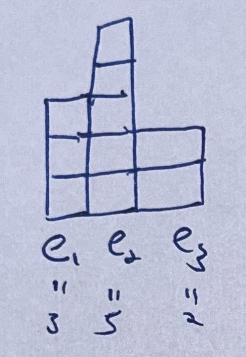
\includegraphics[width=0.15\textwidth]{./img/multi-1.png} 
        \end{figure}
        \item 按勒贝格积分思想,横着计算,第一步计算$g_2*g_2$,第二步计算$\alpha = g_2*g_1$,第三步计算$\beta = \alpha * g_3$,第四步计算$\gamma = \beta * \beta$,第五步计算$\beta * \alpha$, 第六步计算$(\beta * \alpha) * (g_2*g_2)$,总共进行6步乘法操作。
        \begin{figure}[H]
            \centering
            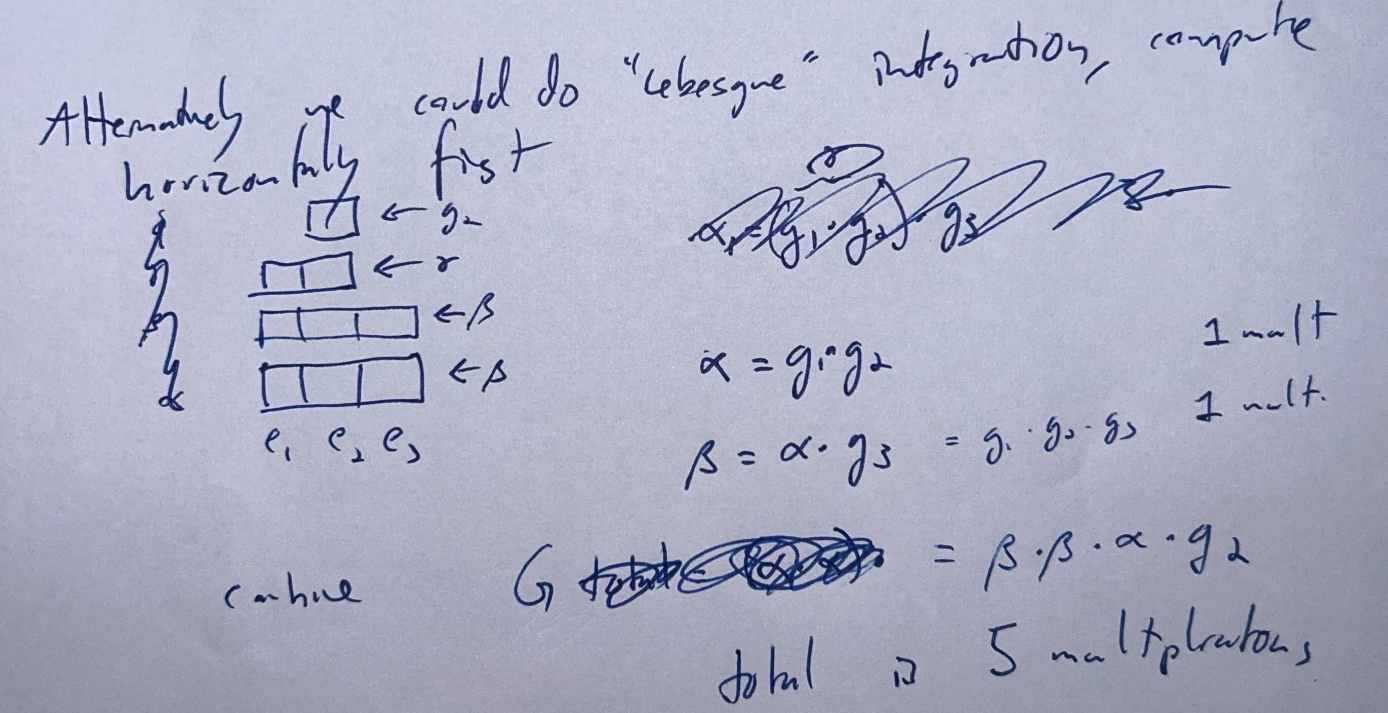
\includegraphics[width=0.9\textwidth]{./img/multi-2.png} 
        \end{figure}
    \end{itemize} 
\end{itemize}
计算$g_1^{2^k}g_2^{2^k} \cdots g_n^{2^k}=(g_1g_2 \cdots g_n)^{2^k}$,先计算括号里的乘积$g_1g_2 \cdots g_n$,也就是$n-1$次乘法,再将结果进行平方,$k$次平方,总共进行$n - 1 + k$次乘法操作。

假设$\mathbb{G}$是一个$p$阶循环群,其中$p$是一个$\lambda$-位素数,设$\lambda = 256$.计算
$$
G = \prod_{i = 0}^{N-1}g_i^{e_i},
$$
其中$e_i$是整数。假设$\lambda \ge N$并且将$\lambda$分解成$s$个legs,即$\lambda = s \cdot t$,例如$\lambda = 256, s=4$,$t=64$,$N=16$.(一般取$s \approx \sqrt{\frac{\lambda}{N}}$,且$t = \sqrt{\lambda N}$)

令$e_i = \sum_{l=0}^{\lambda - 1}e_{i,l} \cdot 2^l$($e_{i,l} \in \{0,1\}$,也就是将$e_i$写成二进制形式).将$\lambda$分解成$s$条legs,则
$$
e_i = \sum_{j=0}^{s-1} \sum_{k=0}^{t-1}e_{i,j+sk} \cdot 2^{j+sk}
$$
例如$\lambda = 256 = 4 \cdot 64$.
\begin{figure}[H]
    \centering
    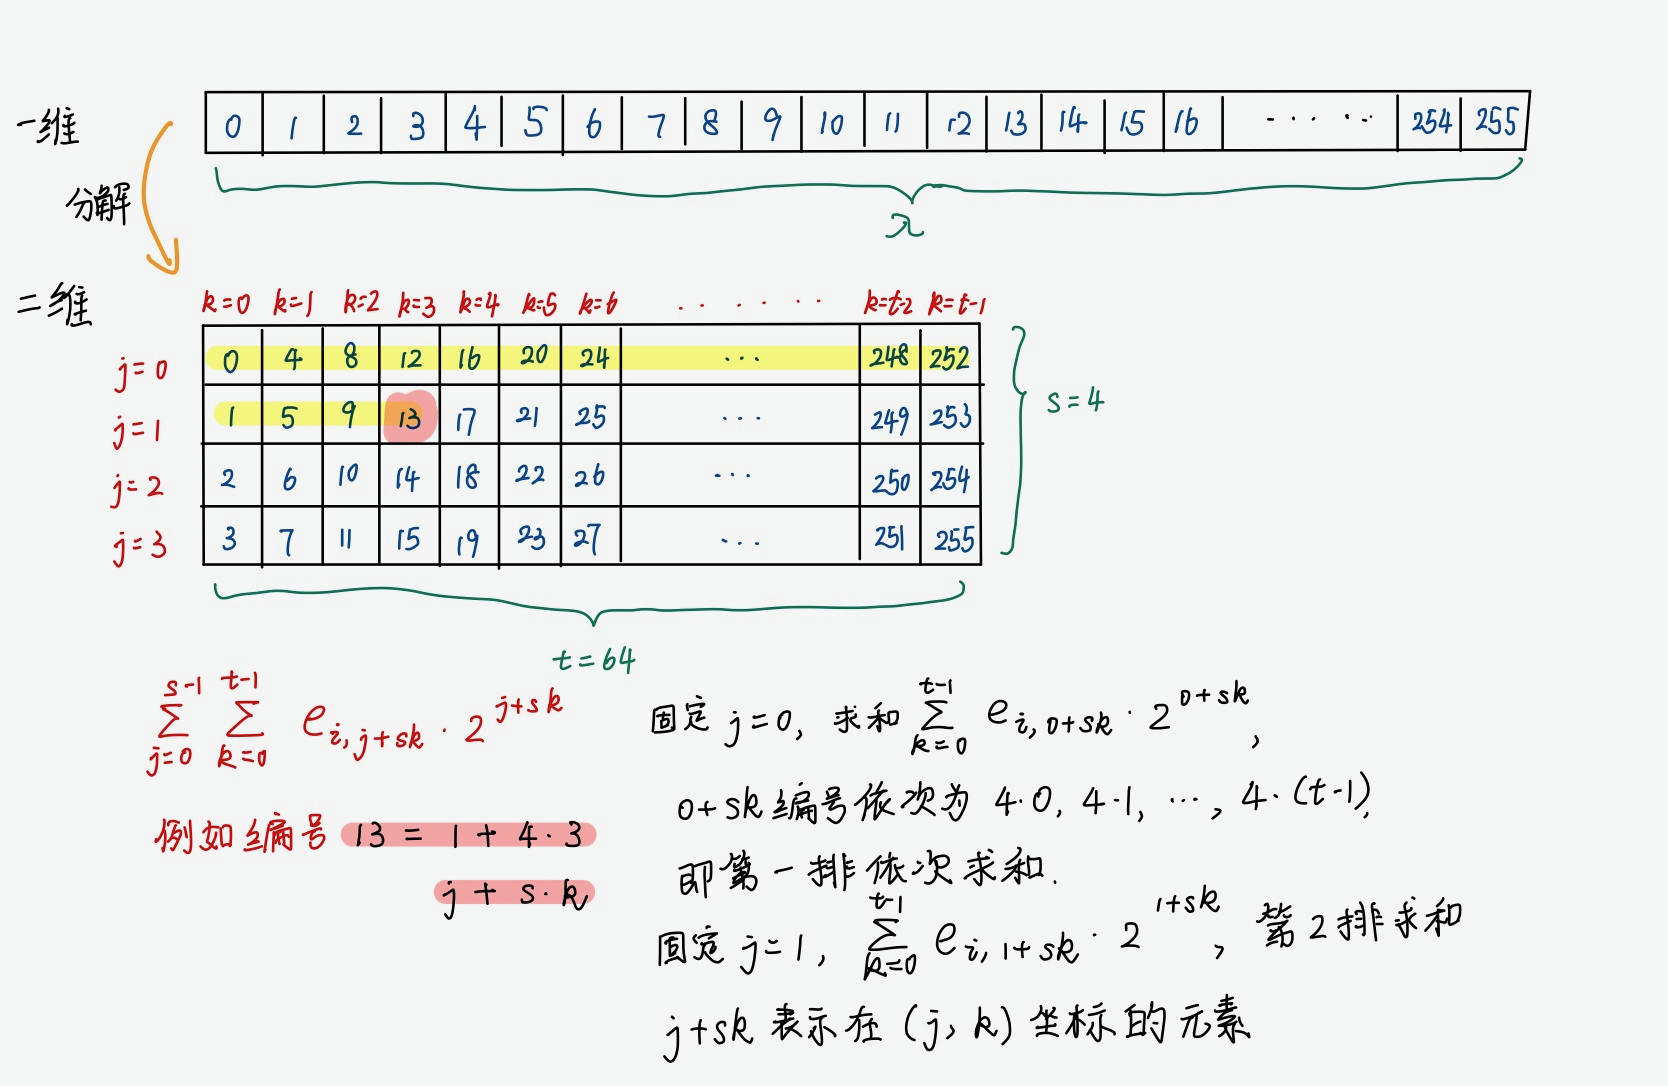
\includegraphics[width=1\textwidth]{./img/sum.png} 
\end{figure}
因此
$$
g_i^{e^i} = \prod_{l=0}^{\lambda -1}g_i^{2^l \cdot e_{i,l} } \overset{\lambda = s \cdot t}{=} \prod_{j=0}^{s-1} \prod_{k=0}^{t-1} g_i^{2^{j+sk} \cdot e_{i,j+sk}},
$$
接着计算$G$
\begin{displaymath}
    \begin{aligned}
        G= \prod_{i = 0}^{N-1}g_i^{e^i} & = \prod_{i = 0}^{N-1} \left( \prod_{j=0}^{s-1} \prod_{k=0}^{t-1} g_i^{2^{j+sk} \cdot e_{i,j+sk}} \right)\\
        & = \prod_{k = 0}^{t-1} \left( \prod_{i=0}^{N-1} \prod_{j=0}^{s-1}  g_i^{2^{j} \cdot e_{i,j+sk}} \right)^{2^{sk}}
    \end{aligned}
\end{displaymath}
记括号里
$$
G_k^{\prime} := \prod_{i=0}^{N-1} \prod_{j=0}^{s-1}  g_i^{2^{j} \cdot e_{i,j+sk}}.
$$
将每一个$i=0,1,\cdots,N-1$依次从上到下排列,最终的结构如下:
\begin{figure}[H]
    \centering
    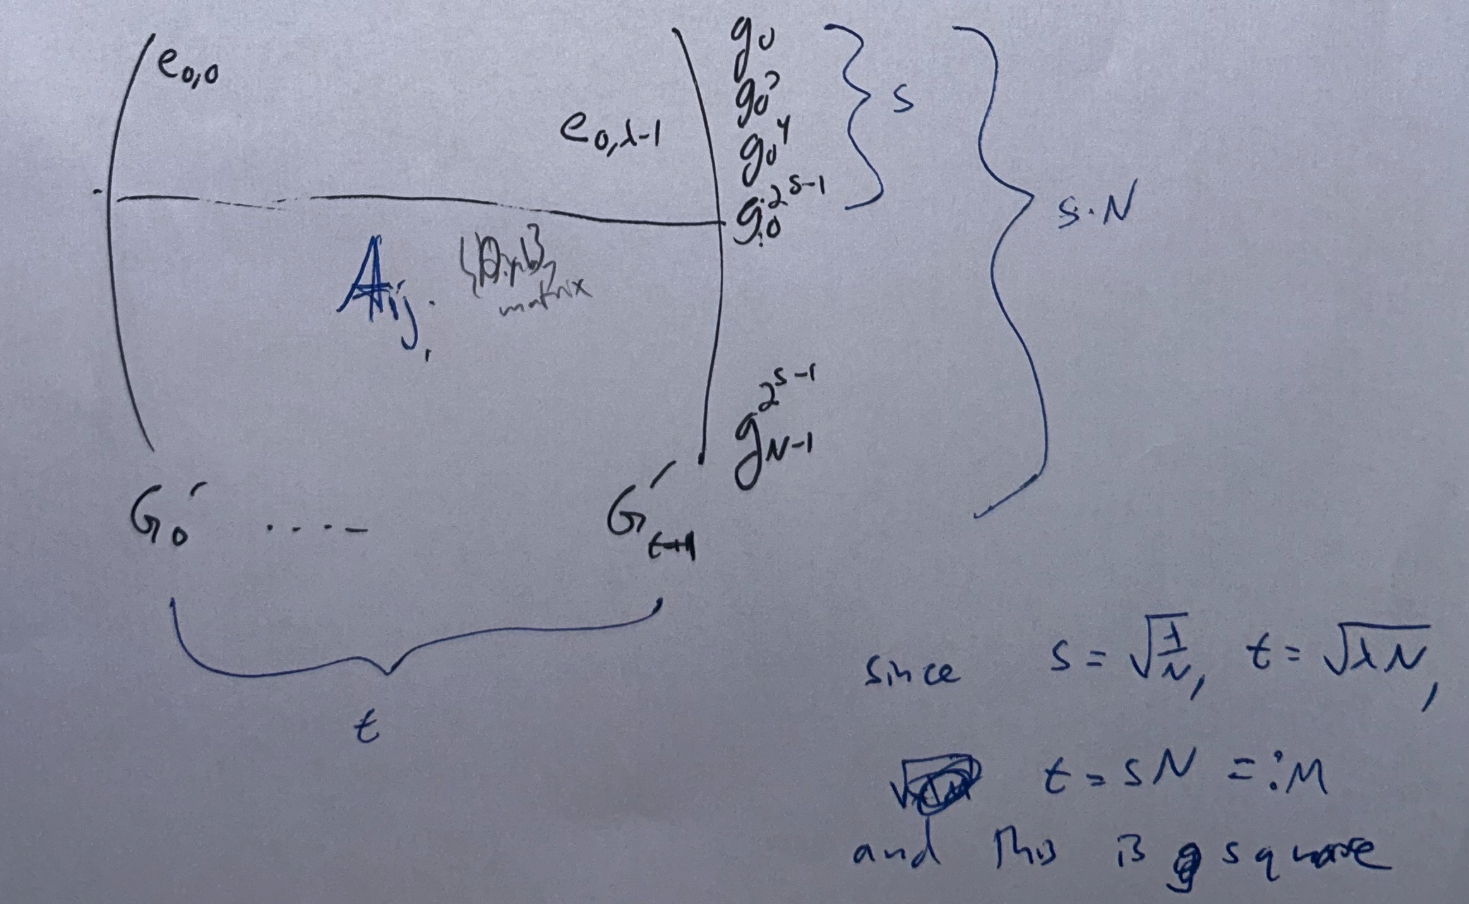
\includegraphics[width=1\textwidth]{./img/matrix.png} 
\end{figure}
每一个$G_k^{\prime}(k = 0, 1, \cdots t-1)$就是竖着的一整列。对于每一个$G_k^{\prime}$乘积内部$g_i^{2^{j} \cdot e_{i,j+sk}}$,需要计算下面这些项:
$$
g_i,g_i^2,g_i^4, \cdots, g_i^j, \cdots,g_i^{2^{s-1}}
$$
总共有$N$个这样的乘积$G_k^{\prime} := \prod_{i=0}^{N-1} \left(\prod_{j=0}^{s-1}  g_i^{2^{j} \cdot e_{i,j+sk}}\right)$,因此总的花销是$N * s = N * \sqrt{\lambda / N} = \sqrt{\lambda N}$.

更一般地,将列向量中的元素分成多个块,每块中至多有$b$个元素。如果列向量中总共有$M$个元素,则将列向量最终分为$S_0, \cdots, S_{\frac{M}{b}-1}$。对于每一个$S_i$,计算$S_i$中所有可能的乘积,记为$T_i$.例如$b=3$,则$S_0=\{h_0,h_1,h_2\},T_0=\{h_0,h_1,h_2,h_0h_1,h_0h_2,h_1h_2,h_0h_1h_2\}.$
\begin{itemize}
    \item 每个$S_i$中有$b$个元素,所有可能的乘积$T_i$中有$2^b$个元素。总共有$M/b$个集合,因此所有集合中乘积有$\frac{2^bM}{b}$个。
    \item 每列有$M/b$个$T_i$,有$M$列,总共有$\frac{M^2}{b}$个$T_i$.
    \item $G_k^{\prime}$中,列向量划分后,每个$S_i$中有$b=s$个元素,一列有$M = s \cdot N$个元素,有$M$列,设置$t = M = s \cdot N$,形成一个方阵。
\end{itemize}

刚刚计算了每个$G_k^{\prime}$,最后要计算
$$
G = \prod_{k = 0}^{t-1} (G_k^{\prime})^{2^{sk}}
$$
\begin{figure}[H]
    \centering
    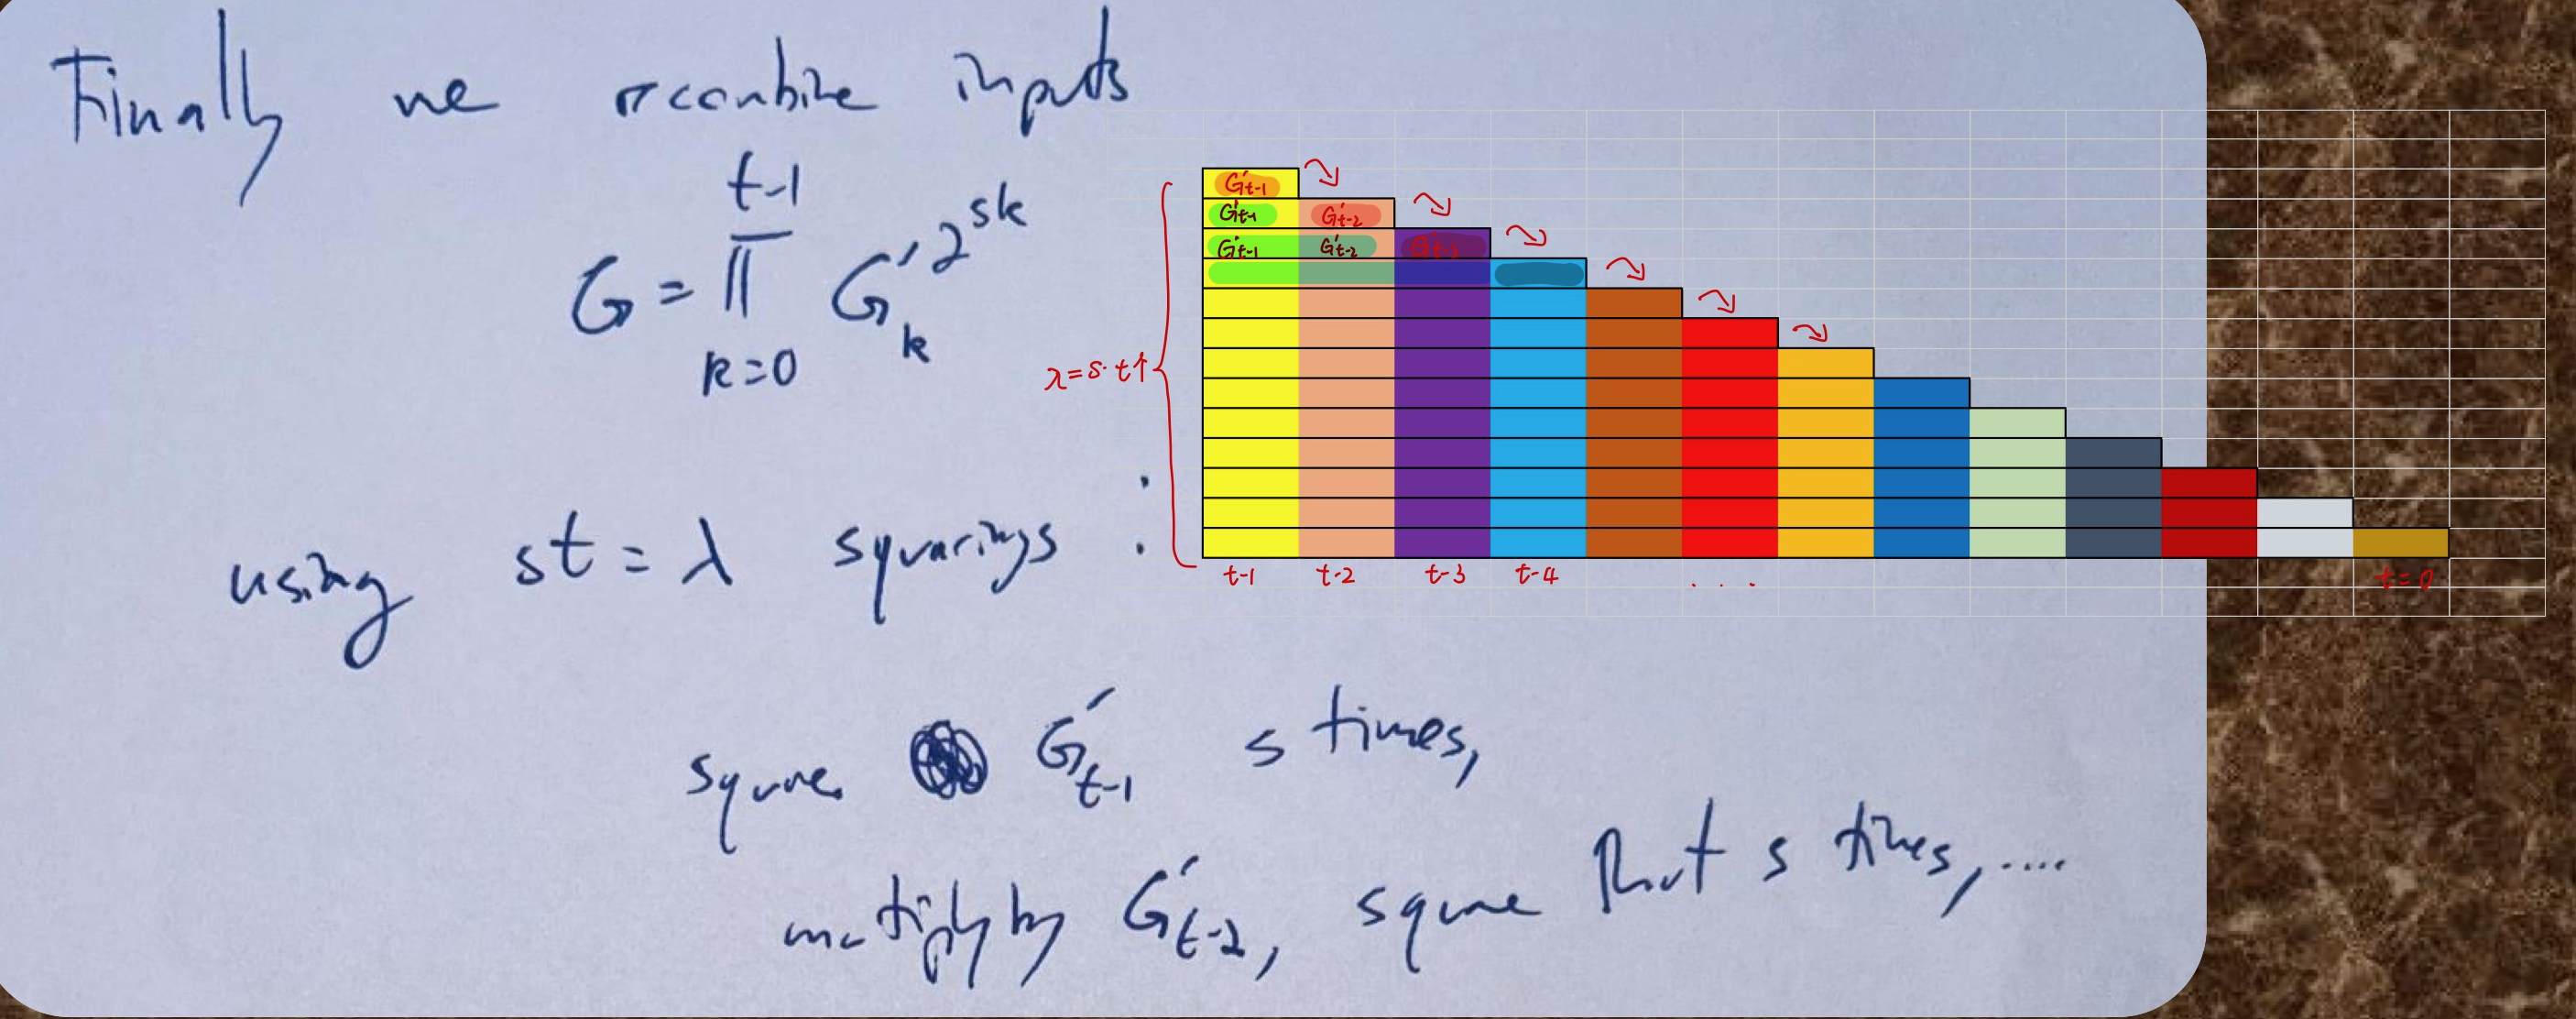
\includegraphics[width=1\textwidth]{./img/G.png} 
\end{figure}
计算$G = \prod_{k = 0}^{t-1} (G_k^{\prime})^{2^{sk}} = \prod_{k = 0}^{t-1} \left((G_k^{\prime})^{2^s}\right)^k$,具体为:
\begin{enumerate}
    \item $ans_{t - 1} = \left(G_{t-1}^{\prime}\right)^{2^s} * \left(G_{t-2}^{\prime}\right)^{2^s}$ 
    \item $ans_{t-2} = ans_{t - 1} * \left(G_{t-3}^{\prime}\right)^{2^s} = G_{t-1}^{\prime} * \left(G_{t-2}^{\prime}\right)^{2^s} * \left(G_{t-3}^{\prime}\right)^{2^s}$ 
    \item $ans_{t-3} = ans_{t - 2} * \left(G_{t-4}^{\prime}\right)^{2^s} = G_{t-1}^{\prime} * \left(G_{t-2}^{\prime}\right)^{2^s} * \left(G_{t-3}^{\prime}\right)^{2^s} * \left(G_{t-4}^{\prime}\right)^{2^s}$ 
    \item $\cdots$
    \item $ans_{1} = ans_{2} * \left(G_{0}^{\prime}\right)^{2^s} = G_{t-1}^{\prime} * \left(G_{t-2}^{\prime}\right)^{2^s} * \left(G_{t-3}^{\prime}\right)^{2^s} * \left(G_{t-4}^{\prime}\right)^{2^s} * \cdots * \left(G_{1}^{\prime}\right)^{2^s} * \left(G_{0}^{\prime}\right)^{2^s}$ 
    \item $G = ans_{t-1} * ans_{t-2} * \cdots * ans_{2} * ans_{1}$
\end{enumerate}
先对$G_{t-1}^{\prime}$进行$s$次平方操作,再乘以$\left(G_{t-2}^{\prime}\right)^{2^s}$,以此类推。这里每个$\left(G_{k}^{\prime}\right)^{2^s}$进行$s$次平方操作,总共有$t$个,因此进行$\lambda = s * t$次平方操作。总共有$t = M$次乘法操作\mnote{在上述第6步中要将乘法结果相乘,不应该是$t + (t - 1)$次乘法操作吗?}。

由于$M = \sqrt{\lambda N} = t = sN$,总共计算次数为:
\begin{figure}[H]
    \centering
    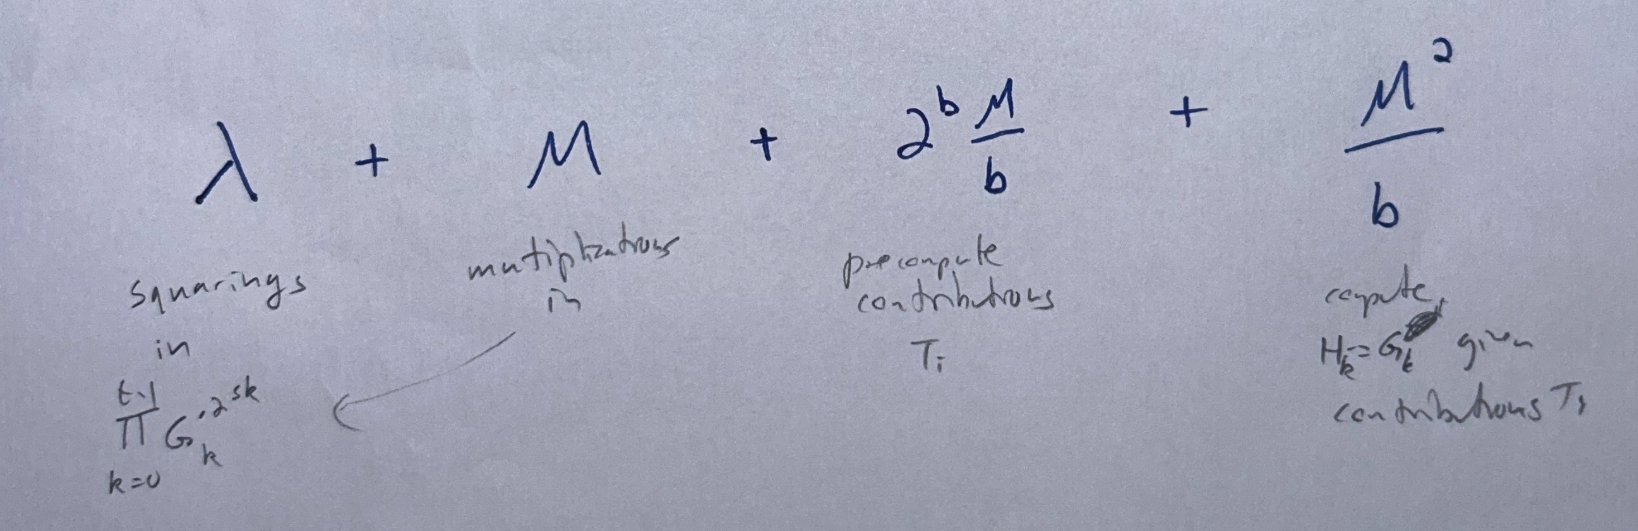
\includegraphics[width=1\textwidth]{./img/operates.png} 
\end{figure}
上述式子中$b$是参数,通过求极小值方法,确定$b$的最优值,即
$$
b = \log M - \log \log M,
$$
将$b$的值代入得
\begin{displaymath}
    \begin{aligned}
         & \lambda + M +  2^b \frac{M}{b} + \frac{M^2}{b} \\
         & \quad = \lambda + M +  2^b \frac{M^2}{\left(\log M - \log \log M\right)\left(\log M\right)} + \frac{M^2}{\log M - \log \log M} \\
         & \quad = \lambda + (1 + o(1))\frac{M^2}{\log M} \\
         & \quad = \lambda + (1 + o(1))\frac{\lambda N}{\log \lambda N} \quad \quad(M = t = \sqrt{\lambda N}).
    \end{aligned}
\end{displaymath}
\end{document}